\documentclass[a4paper, 11pt]{article}
\usepackage[titles]{tocloft}
\usepackage[utf8]{inputenc}
\usepackage{natbib} % eksempel til sitering: \cite{bass2003software}. referanser legges i ref.bib. Etter å ha oppdatert ref.bib må bibtex ImplementationDocument.aux kommando kjøres. 
\usepackage{hyperref}
\usepackage[pdftex]{graphicx}
\usepackage{algorithmic}

%\usepackage{amssymb,amsmath}



\newcommand{\HRule}{\rule{\linewidth}{0.5mm}}

\title{\textbf{Action Hero Defense}\\\HRule\\Architectural Description\\ Group 23}
\author{\and Håvard Geithus
	\and  Sondre Løberg Sæter 
	\and Nicolai Meltveit 
	\and Hallvard Andreas Eriksen 
	\and  Håkon Drolsum Røkenes}
\date{\today}

\begin{document}

%\maketitle

\begin{titlepage}
\begin{center}

\vspace{10 mm}
{ \huge\bfseries Warcraft TD}\\[0.4cm]
Architectural Description\\
Group 23
\begin{figure}[h]
	\center
	
\includegraphics[scale=2]{images/peons}
\end{figure}

\vfill
\begin{minipage}{0.4\textwidth}
\begin{flushleft} \large
\emph{Authors:}\\
Håvard Geithus\\ 
Sondre Løberg Sæter\\ 
Nicolai Meltveit\\
Hallvard Andreas Eriksen\\
Håkon Drolsum Røkenes\\
\end{flushleft}
\end{minipage}
\begin{minipage}{0.4\textwidth}
\begin{flushright} \large
\emph{COTS:} Android-SDK \vspace{5 mm}

\emph{Quality Attributes:} \\

Modifiability\\ Testability\\ Usability
\end{flushright}
\end{minipage}
\vspace{10 mm}







%\vfill

% Bottom of the page
{\large \today}



\end{center}
\end{titlepage}

\renewcommand\thepage{}
\tableofcontents
\clearpage
\listoffigures
\clearpage

\renewcommand\thepage{\arabic{page}}
\setcounter{page}{1}
\section{Introduction}
This report will give an overview over the chosen architectures of the Action Hero Defense game, developed as a part of the TDT4240 course assignment.
We will focus on the reasons behind our choices of architecture, in addition to discussing how the chosen architecture conforms to the quality requirements which are set. Primarily the modifiability and testability quality requirements.

In the first section of this report, we will give an introduction on the architectural drivers of the game. This section will describe how the both the functional and quality requirements influence our choice of architecture. 

The next section, the architectural views, will offer a description of the architecture from different perspectives, or \emph{views}. Here we focus on two perspectives which we feel is most relevant for our project; the logical and the development view.

The Tactics-section will focus on the various techniques and methods we will employ to obtain the desired quality requirements, such as the modifiability 


Finally, we will discuss the design and architectural patterns we wish to implement in our system. We have decided on the Model-View-Controller architectural pattern and we will discuss how this pattern fits in to our selected quality requirements.


\section{Design Details}


\subsection{Menu Description}
When the game is started, the user is presented with a menu. The layout for the menu is defined with a layout XML-file. Using XML is the most common way to control layout for Android applications.\cite{android:ui} This menu is represented programitically with the MenuActivity class, which extends the Activity class. An activity in Android is in most cases "what you see", and defines where the user is in the application. A user can navigate between activities through the use an Activity stack, which defines the most recent activities, thus allowing to navigate backwards. This is generally done with the "back" button on the phone, or customized buttons/events introduced by the developer of the application.\cite{android:activity}

The menu activity consists of a "Play" button, which starts the game. When this button is pressed, a new activity is started -- PlayActivity. This activity starts the game. When the player has died, or has pressed the back button, PlayActivity is paused, and MenuActivity is resumed. This can be further explained with the Activity lifecycle in figure ~\ref{fig:activityLifecycle}, which is provided by the Android Developer Guide.


\begin{figure} [h]
	\center
		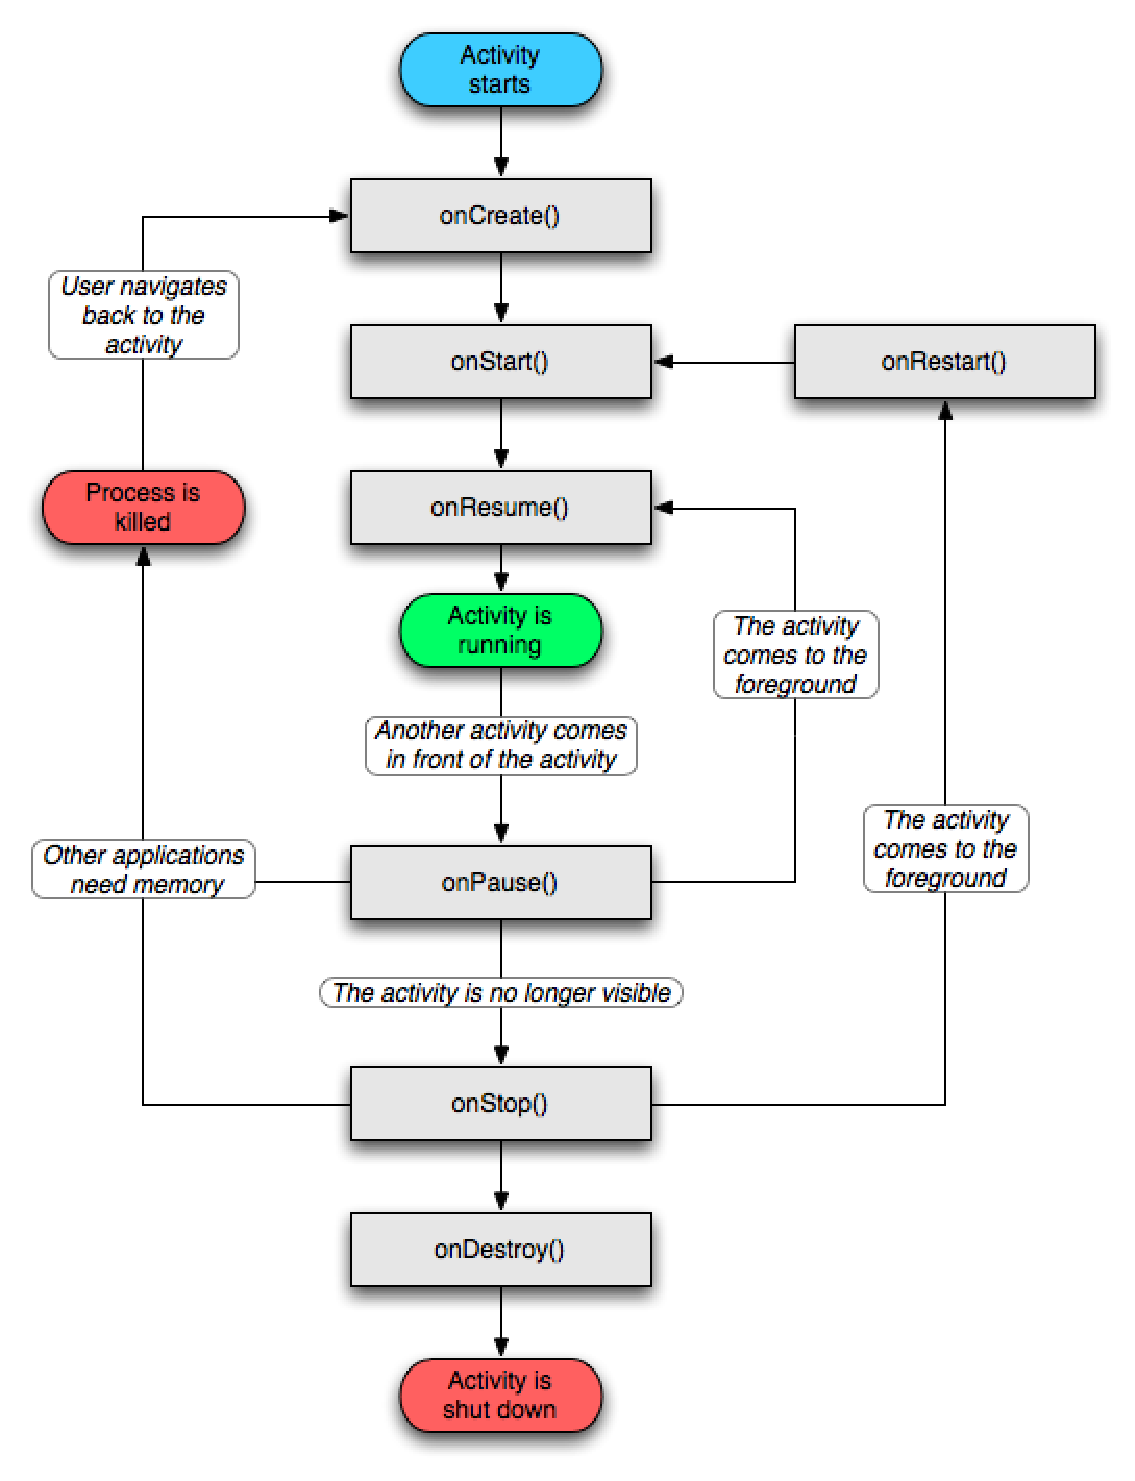
\includegraphics[scale=0.5]{main/figures/activity_lifecycle}
		\caption{Activity Lifecycle\cite{android:activity}}
		\label{fig:activityLifecycle}
\end{figure}

\subsection{Game Description}
When PlayActivity is started from the menu, the game starts. Upon creating the activity, onCreate is called and initializes our game object, as explained in figure \ref{fig:activityLifecycle}. The game object consists of a state, which again consists of different layers. Figure \ref{fig:structure} displays an overview over the most important components of the game. 

The view of the game is displayed using the Sheep framework, through the use of a canvas, which decide what is shown on the display. The game object calls the update and draw methods frequently, thus allowing animation and movement. The update and draw methods are called in a chain downwards in the hierarchy of classes, which are further explained in the architectural report.\cite{arcReport}

\subsection{Touch Gestures}
The GestureController class listens for touch gesture made by the user. The gestures detected are pinch zoom (two fingers moving away or towards each other) and long press. When initiating a pinch zoom, the canvas is enlarged through the scale method. When a long press is detected, a dialogbox to create tower will appear. The dialog layout is defined in a XML layout file. After clicking on a tower, the tower will be placed at the position which the long press appeared.

The user will not be able to zoom in more than 3 times normal zoom level, and out more than the size of the map, which is the starting zoom level for any screen. The zoom level is calculated with the formula in equation \ref{eq_zoom}. If the user tries to zoom outside these values, the zoom level will be set to the respective max or min level.


\begin{equation}\label{eq_zoom}
	\frac{displaysize}{mapsize} < zoom level < 3
\end{equation}

\subsection{Music}
Music is played through the use of the MediaPlayer class, which is initiated when PlayActivity is started/resumed, and paused when the game is no longer in focus.

\subsection{Tiled Map}
A lot of the modifiability requirements are concerned about game content. One should be able to change, add or delete content with ease. In the context of the game map, this means that a map editor should be availible for the map designers. Hard-coding a map directly into the programming language is out of the question. Furthermore, the map should be stored in a flexible data format which is easy processs programatically. 

These goals are achieved by basing the map functionality on the Tiled Map Editor.\cite{mapeditor} It is an open source, general purpose map editor, which handles maps stored in the XML data format\footnote{The file extension is *.tmx}. It is written in C++ using the Qt application framework, but it is also ported to Java\footnote{The Java version is no longer maintained officially}, which is what we used. Unfortunately, the code had a lot of dependencies on the Swing API, and this is not a part of the Android API. In other words, the functionality had to be ported to Android. Only a subset of the functionality was ported to the application; about 60\% of the original code. This means that the map has to be designed on a desktop computer running a standard Java Virtual Machine (JVM), and the produced *.tmx file can then be read (parsed) on the Android Dalvik Virtual Machine (supporting the Android API).

\subsubsection{Creating And Parsing Map}\label{parsingmap}
A game map is 2-dimensional and composed of small square images called tiles. The map itself is referred to as a tiled map. In order to create a map, one first needs a tile set. This is basically a single image file which is constructed as a regular grid of smaller images. This image is then cut along the grid lines into separate images. All of these new images constitutes the palette from which one can draw the map. This functionality resides in the Tiled Map Editor. In addition to drawing tiles, one can draw objects. These are typically not rendered, but only used as logical elements. This was used to define spawn, goal and waypoint areas in the map. With this, the map design process has become rather effortless and the dataformat is very flexible. The map creation process was considered as satisfactory.

Representing arbitrary data structures with XML is easy, interpreting and parsing them is another story. The *.tmx files are structured as a tree. The DOM (Document Object Model) parser library was used to parse the map files. \cite{dom}


\subsection{Enemies}

The enemies in the game consists of streams of sprites moving from the spawn-area of the map in a set path to the goal-area of the map. There are four types of enemies, illustrated in figure \ref{fig:enemies}

\begin{figure}[htbp]
	\centering
		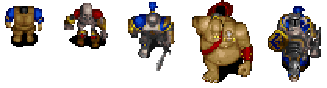
\includegraphics{main/figures/enemies}
	\caption{Enemies}
	\label{fig:enemies}
\end{figure}


An enemy is represented as an EnemySprite-object, which extends the class Sprite from the Sheep-framework. The Sprite-class contains functionality for drawing and updating a sprite on the screen. It also contains functions for setting an image as the visual representation, as well as functions for moving the sprite around the screen. 

In addition to the functionality already implemented in the Sprite-class, the EnemySprite contains properties such as hit-points, its status (when the hitpoints are dropped below zero, the sprite is considered dead), as well as information regarding the sprite's position on the map. It also has a visiblity-property, deciding whether the sprite should be visible on the screen. 

\subsubsection{Pathing}
As mentioned in section \ref{parsingmap}, the game maps contain information about spawn, goal and waypoint areas. Even information about which areas are walkable is coded into the map. This information is handled by the TowerDefenseMapLayer class. To construct a path, the elements are first ordered like this: $spawn, waypoint_1, waypoint_2, ..., waypoint_n, goal$. Then it is iterated over in this order, building a path between every two consecutive elements, and linking these paths together. The algorithm used is the A* search algorithm \cite{aima}, and the admissible heurestic is the manhattan distance \cite{wiki:manhattan}.

\subsection{Towers}
The towers are sprites of the type TowerSprite-object, and they extend the Sprite-class, just like the enemies. The difference between the towers and the enemies is that the towers does not move after they are spawned. Instead, the towers have an attack-animation which is performed in the same way as the animation for the enemies. The player can create four different towers in the game, which are illustrated in figure \ref{fig:towers}. 

\begin{figure}[htbp]
	\centering
		
\includegraphics{main/figures/towers}
	\caption{Towers}
	\label{fig:towers}
\end{figure}


All towers have different range, damage and price, which are defined in a class called "Globals". By having a Globals class with all the properties of each tower one can easily change the difficulty of the game, in order to achieve balance in the gameplay.


The towers frequently check for enemies in near proximity, and shoots if possible. The shooting functionality is further explained in detail by the following pseudocode.\newline


\begin{algorithmic}
\FORALL{Towers}
	\IF{Tower.isFiring}
		\IF{Tower.getTarget.isDead}
			\item Stop firing
		\ELSIF{\NOT targetInRange}
			\item Stop firing
		\ELSE
			\item Keep firing at target
		\ENDIF
	\ELSE
		\FORALL{enemies}
			\IF{targetInRange(tower, enemy) and \NOT enemy.isDead}
				\item Fire at enemy
				\item Stop looping through enemies
			\ENDIF
		\ENDFOR
	\ENDIF
\ENDFOR
\end{algorithmic}

Here the list of towers is iterated through, checking if it should change target or not. When checking for a new target, the list of enemies is iterated through. The first enemy of the list is chosen, then the for loop is stopped. Since the first enemy in the list is chosen, the enemy closest to the goal is chosen. The targetInRange function is calculated with the formula explained in equation \ref{eq:targetInRange}. When iterating through the tower and enemy lists, synchronized is called on both lists, to lock the access to these lists to the current thread. This is further explained in section \ref{threading}.

\begin{equation}\label{eq:targetInRange}
	(TowerX - enemyX)^2 +(TowerY - EnemyY)^2 <= tower range^2
\end{equation}

Here X and Y refers to the coordinates of the towers and enemies, while tower range refers to the range of the different towers.

\begin{figure}[htbp]
	\centering
		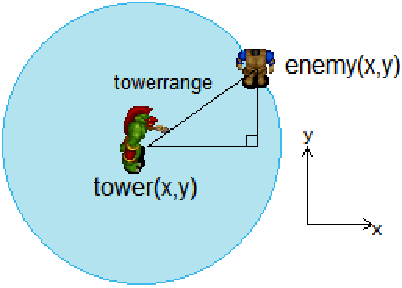
\includegraphics{main/figures/range}
		\caption{Attack range of an axe thrower}
	\label{fig:range}
\end{figure}

Figure \ref{fig:range} shows an example of the attack range of the axe thrower tower.


\subsubsection{Animation}

By adding several images, the sprite can be animated. In our case the sprite has images which makes the sprite seem as it is walking and attacking, as illustrated in figure \ref{fig:axeanimation}. Animation is accomplished by switching the image giving the visual representation of the sprite in a set frequency. 

\begin{figure}[htbp]
	\centering
		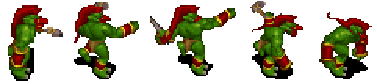
\includegraphics{main/figures/axeanimation}
		\caption{Axe thrower attack animation}
	\label{fig:axeanimation}
\end{figure}


The images of a EnemySprite-object is collected in an EnemyImageStructure-instance. This is a structure containing all the images connected to a sprite, including five animation images and an image illustrating that the sprite is dead.



\section{User Manual}
This section will give a tutorial in how to use or modify the application. 

\subsection{User Level}
From a users point of view this tutorial will cover menu’s and how to play the game. 
\clearpage
\subsection{Main Menu}

When the application is launched, the main menu will appear. Here you have three buttons, as shown in figure \ref{usermanual:menu}

\begin{figure} [h]
	\center
		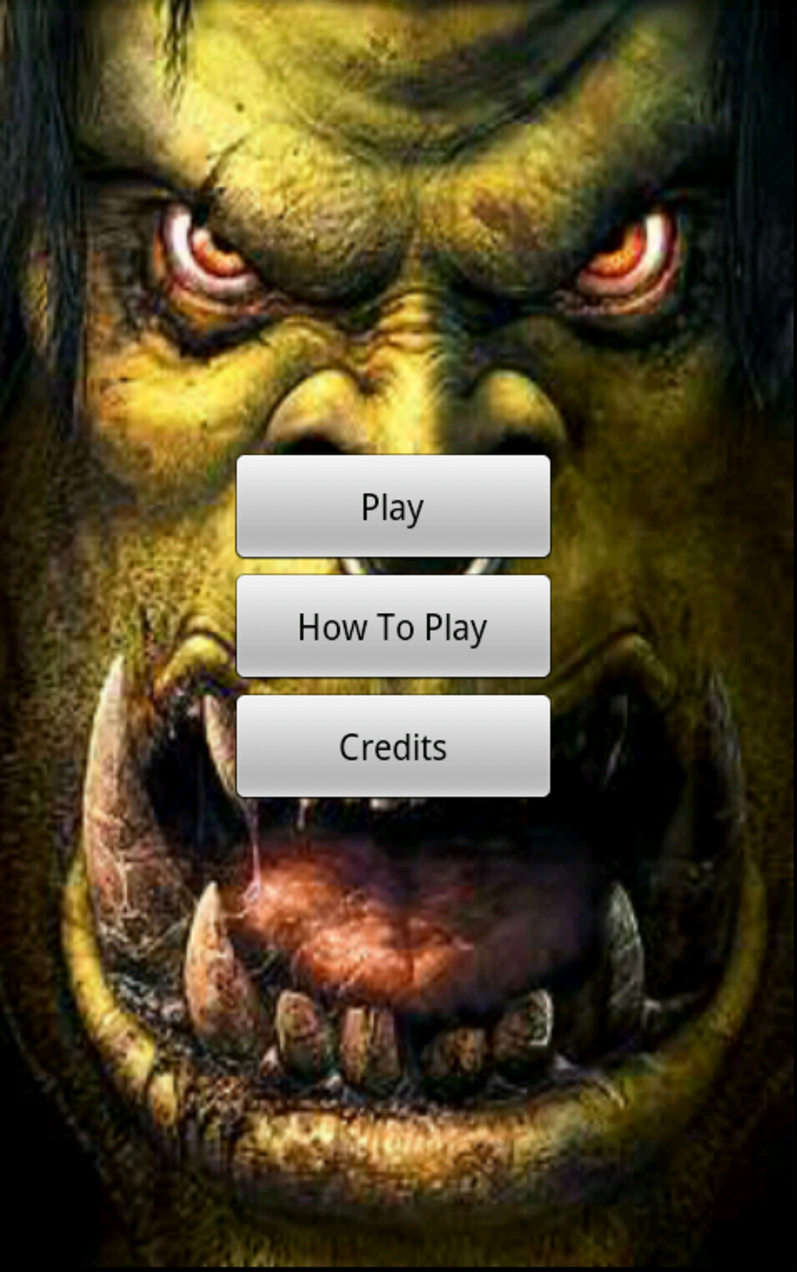
\includegraphics[scale=0.5]{main/figures/screenshots/menu}
		\caption{Main Menu}
		\label{usermanual:menu}
\end{figure}

The options you have when in the main menu is:

\begin{itemize}
	\item Play -- pressing this button will start the game
	\item How To Play -- If you press this button you will get a fast tutorial on how to play the game.
	\item Credits -- The credits will be displayed
\end{itemize}



\subsection{The Game}
You have pressed the “Play” button, and the game have now started. The first wave will after a little while start to appear, and you shall kill it by building towers.

The mobs will be walking on a brown dirt road, while the empty green fields can be used for tower building. Figure \ref{usermanual:startGame} shows how the start of the game looks like.

\begin{figure} [h]
	\center
		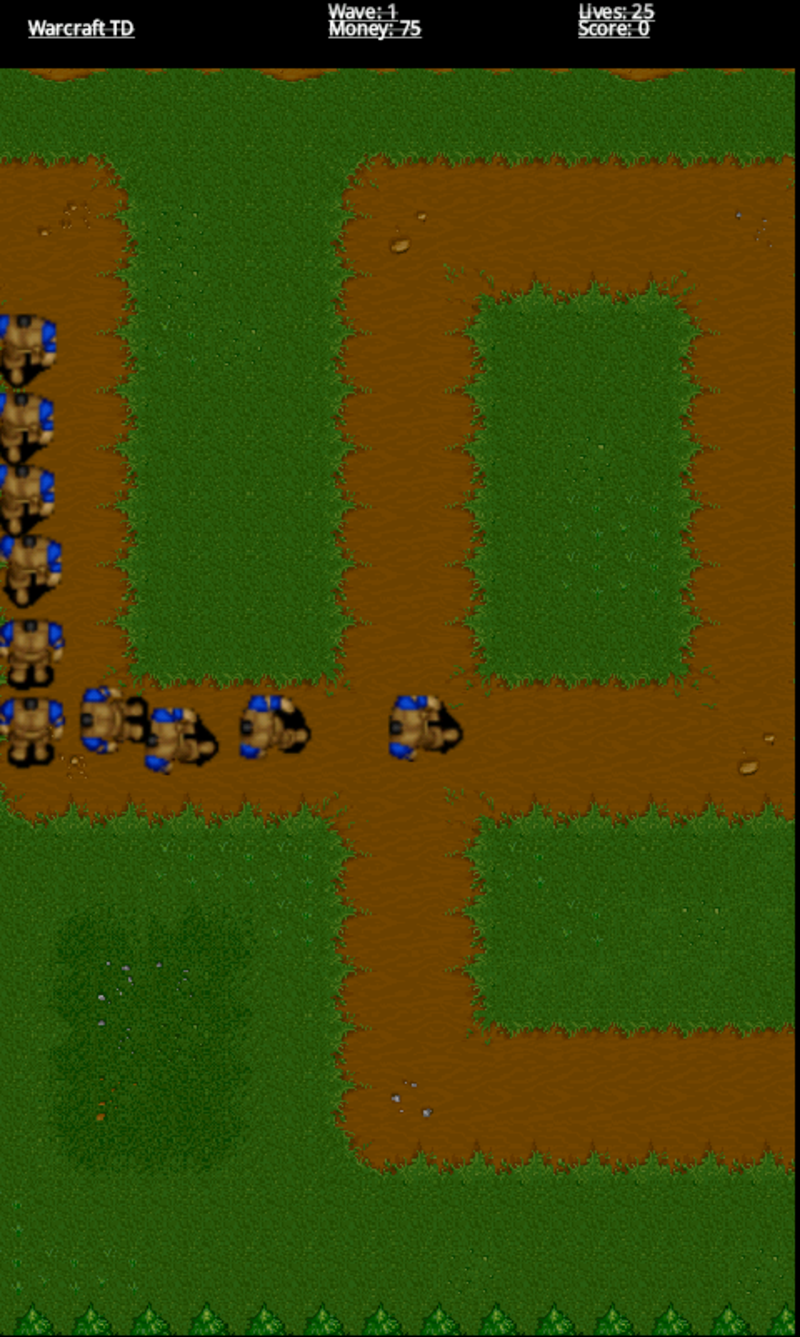
\includegraphics[scale=0.5]{main/figures/screenshots/play}
		\caption{Start of game}
		\label{usermanual:startGame}
\end{figure}

\subsection{Building Towers}
When the game has started you can start building your first tower. To get the Tower Menu to appear, you need to press the spot you want to build a tower, and hold for one second. When the Tower Menu appears, you choose which tower to build by clicking the chosen tower. If you don’t have enough resources for a special tower, that tower will be grayed out in the dialog. Figure \ref{usermanual:createTower} shows how the dialog looks like.

\begin{figure} [h] 
	\center
		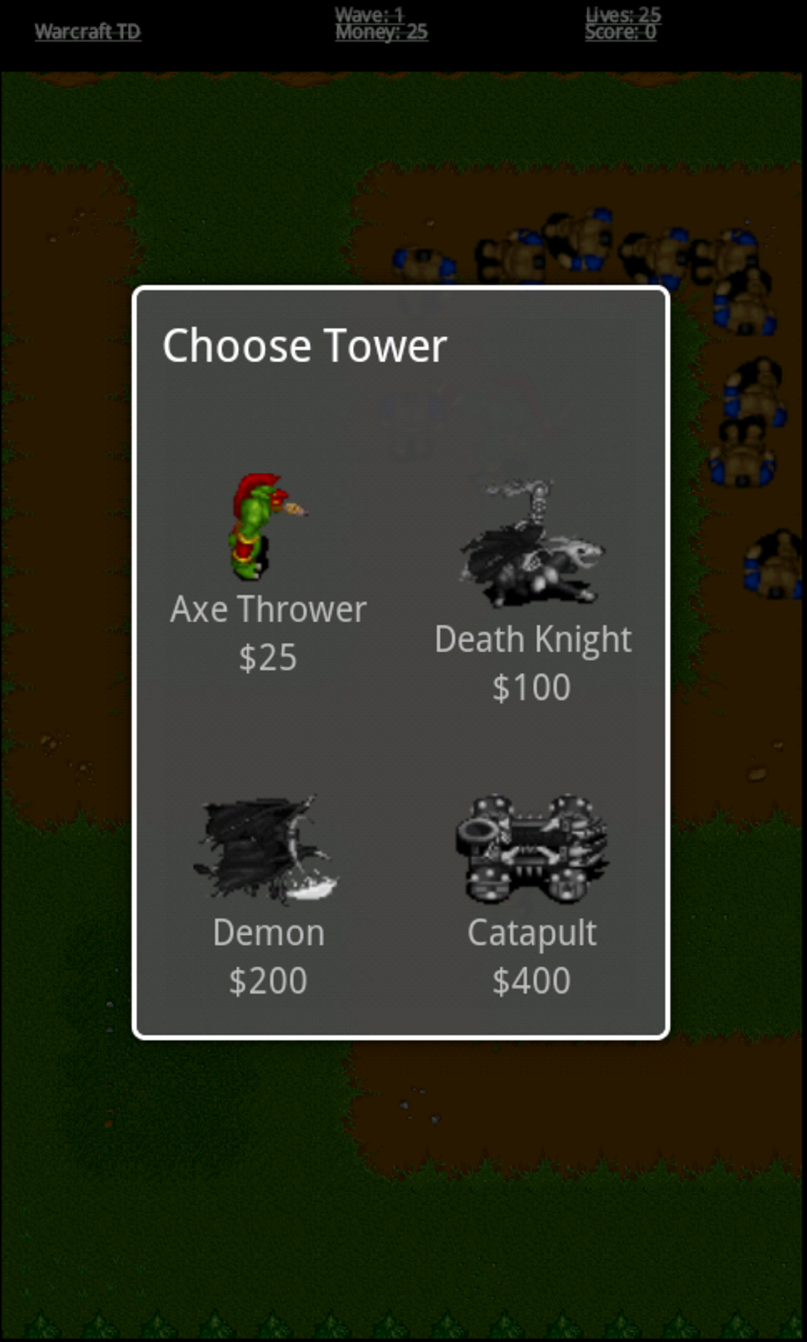
\includegraphics[scale=0.5]{main/figures/screenshots/create_tower}
		\caption{Create Tower Dialog}
		\label{usermanual:createTower}
\end{figure}

There are four different types of towers. The towers have increasing range and damage, aswell as price. 

\begin{itemize}
	\item Axe Thrower: A tower dealing minor damage
	\item Death Knight: A tower dealing medium damage
	\item Demon: A tower dealing high damage 
	\item Catapult: A tower dealing massive damage
\end{itemize}

Towers should be placed in key positions where they can shoot enemies for the longest time. It is up to the player to decide which positions will give the best results. Figure \ref{usermanual:gameplay} displays the game after placing a couple of towers.
\clearpage
\begin{figure} [h]
	\center
		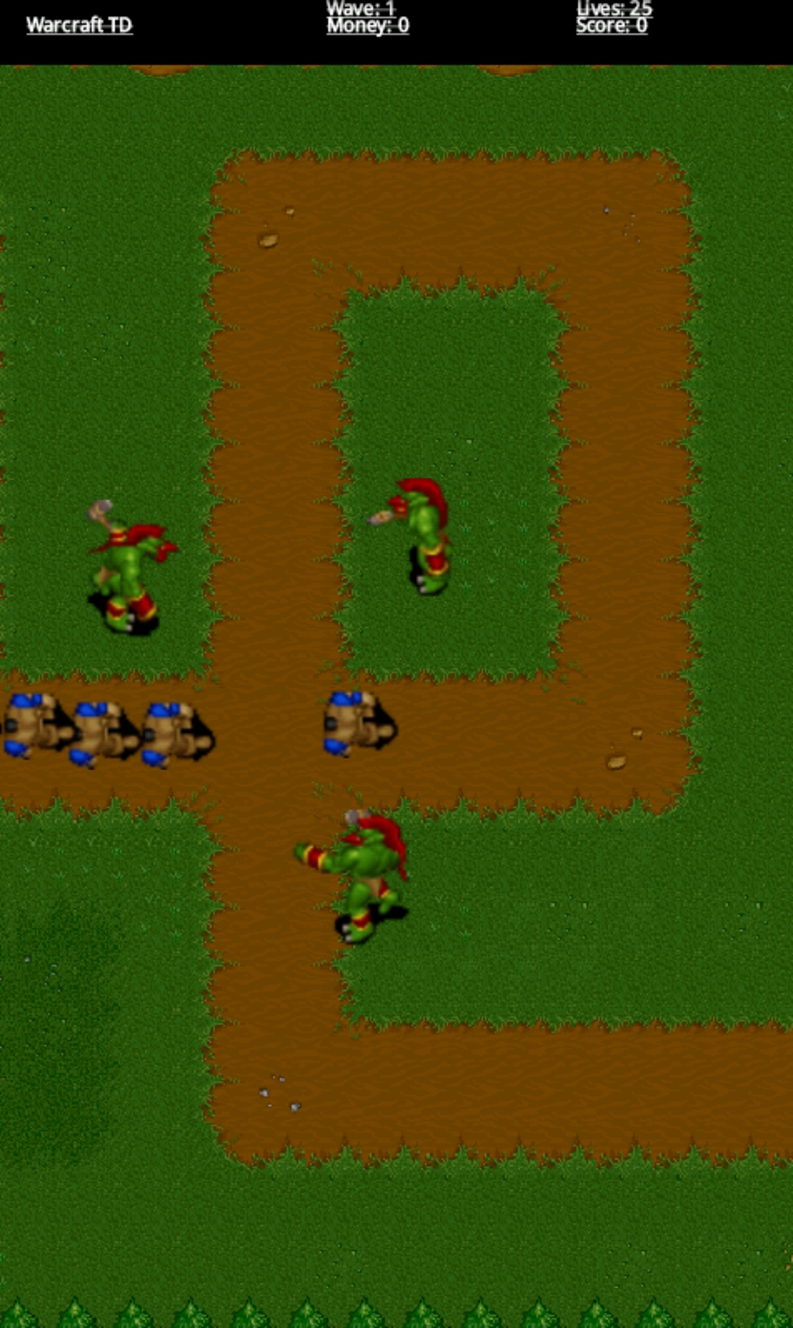
\includegraphics[scale=0.5]{main/figures/screenshots/gameplay}
		\caption{Gameplay}
		\label{usermanual:gameplay}
\end{figure}

%\subsection{Developer Guide}

%Here follows a short introduction on how to the application can be modified.

%All changes to the game has to be done before compilation time. We have tried to make it relatively easy to make changes or additions to the game or its content.

%\subsubsection{Creating a new map}


\section{Test Report}
\subsection{Functional Requirements}
The following section contains the test reports that was made when the game was tested. The tests were performed in the game, and each test had a concrete objective of what to test.

  \begin{tabular}{|l | p{10cm} | }
	\hline	
	\textbf{Type} & \textbf{Info} \\
	\hline
	FR.1 & Stop mobs using towers \\
	\hline
	Priority & High  \\
	\hline
	Executor & Sondre  \\
	\hline
	Date & 07.04.2011 \\
	\hline
	Time & 15 seconds \\
	\hline
	Evaluation & Success! \\
	\hline
  \end{tabular}
  \\
  \\
  \\  
  \begin{tabular}{|l | p{10cm} | }
	\hline	
	\textbf{Type} & \textbf{Info} \\
	\hline
	FR.2 & Non-overlapping waves \\
	\hline
	Priority & High  \\
	\hline
	Executor & Sondre  \\
	\hline
	Date & 07.04.2011 \\
	\hline
	Time & 1 min \\
	\hline
	Evaluation & Success! \\
	\hline
  \end{tabular}
  \\
  \\
  \\
  \begin{tabular}{|l |p{10cm} |}
	\hline	
	\textbf{Type} & \textbf{Info} \\
	\hline
	FR.3 & Next wave after time period  \\
	\hline
	Priority & High  \\
	\hline
	Executor & Sondre  \\
	\hline
	Date & 07.04.2011 \\
	\hline
	Time & 1 min \\
	\hline
	Evaluation & Success, though time period is only a few seconds. \\
	\hline
  \end{tabular}
  \\
  \\
  \\
  \begin{tabular}{|l |p{10cm} |}
	\hline	
	\textbf{Type} & \textbf{Info} \\
	\hline
	FR.4 & Increasing mob strength\\
	\hline
	Priority & Medium  \\
	\hline
	Executor & Sondre  \\
	\hline
	Date & 07.04.2011 \\
	\hline
	Time & 2 min \\
	\hline
	Evaluation & Success! The mobs have more hit points per level. \\
	\hline
  \end{tabular}
  \\
  \\
  \\
  \begin{tabular}{|l | p{10cm} |}
	\hline	
	\textbf{Type} & \textbf{Info} \\
	\hline
	FR.5 & Earning gold \\
	\hline
	Priority & High  \\
	\hline
	Executor & Sondre  \\
	\hline
	Date & 07.04.2011 \\
	\hline
	Time & 1 min \\
	\hline
	Evaluation & Success! Killing mobs give gold. \\
	\hline
  \end{tabular}
  \\
  \\
  \\
  \begin{tabular}{|l | p{10cm} |}
	\hline	
	\textbf{Type} & \textbf{Info} \\
	\hline
	FR.6 & Winning the game \\
	\hline
	Priority & Medium \\
	\hline
	Executor & Sondre  \\
	\hline
	Date & 07.04.2011 \\
	\hline
	Time & 10 min \\
	\hline
	Evaluation & Success! \\
	\hline
  \end{tabular}
  \\
  \\
  \\
  \begin{tabular}{|l | p{10cm} |}
	\hline	
	\textbf{Type} & \textbf{Info} \\
	\hline
	FR.7 & High score \\
	\hline
	Priority & Low  \\
	\hline
	Executor & Sondre  \\
	\hline
	Date & 04.05.2011 \\
	\hline
	Time & 1 seconds \\
	\hline
	Evaluation & Fail. Not implemented. \\
	\hline
  \end{tabular}
  \\
  \\
  \\
  \begin{tabular}{|l | p{10cm} |}
	\hline	
	\textbf{Type} & \textbf{Info} \\
	\hline
	FR.8 & Player health \\
	\hline
	Priority & High  \\
	\hline
	Executor & Sondre  \\
	\hline
	Date & 07.04.2011 \\
	\hline
	Time & 2 min \\
	\hline
	Evaluation & Success! The player has 25 lives \\
	\hline
  \end{tabular}
  \\
  \\
  \\
  \begin{tabular}{|l | p{10cm} |}
	\hline	
	\textbf{Type} & \textbf{Info} \\
	\hline
	FR.9 & Damage test level \\
	\hline
	Priority & Low  \\
	\hline
	Executor & Sondre  \\
	\hline
	Date & 05.04.2011 \\
	\hline
	Time & 1 seconds \\
	\hline
	Evaluation & Fail. Not implemented. \\
	\hline
  \end{tabular}
  \\
  \\
  \\
  \begin{tabular}{|l | p{10cm} |}
	\hline	
	\textbf{Type} & \textbf{Info} \\
	\hline
	FR.10 & Upgradeable towers \\
	\hline
	Priority & Low  \\
	\hline
	Executor & Sondre  \\
	\hline
	Date & 05.04.2011 \\
	\hline
	Time & 1 seconds \\
	\hline
	Evaluation & Fail. Not implemented. \\
	\hline
  \end{tabular}
  \\
  \\
  \\
  \begin{tabular}{|l | p{10cm} |}
	\hline	
	\textbf{Type} & \textbf{Info} \\
	\hline
	FR.11 & Menu for tower building (Graphical) \\
	\hline
	Priority & High  \\
	\hline
	Executor & Sondre  \\
	\hline
	Date & 07.04.2011 \\
	\hline
	Time & 15 seconds \\
	\hline
	Evaluation & Success. It works as well!  \\
	\hline
  \end{tabular}
  \\
  \\
  \\
  \begin{tabular}{|l | p{10cm} |}
	\hline	
	\textbf{Type} & \textbf{Info} \\
	\hline
	FR.12 & Menu for selling or upgrading towers (Graphical) \\
	\hline
	Priority & Low  \\
	\hline
	Executor & Sondre  \\
	\hline
	Date & 05.04.2011 \\
	\hline
	Time & 1 seconds \\
	\hline
	Evaluation & Fail. Not implemented. \\
	\hline
  \end{tabular}
  \\
  \\
  \\
  \begin{tabular}{|l | p{10cm} |}
	\hline	
	\textbf{Type} & \textbf{Info} \\
	\hline
	FR.13 & Status bar \\
	\hline
	Priority & High  \\
	\hline
	Executor & Sondre  \\
	\hline
	Date & 07.04.2011 \\
	\hline
	Time & 10 seconds \\
	\hline
	Evaluation & Success! \\
	\hline
  \end{tabular}

\subsection{Quality requirements}

In this section the test reports of the quality scenarios are presented. These are both modifiability and testability scenarios. The reports contain what is to be tested, what response is expected from the test, and what response that was actually given.
\\
\\
\\
\begin{tabular}{|l | p{8.7cm} |}
	\hline	
	\textbf{Type} & \textbf{Info} \\
	\hline
	MS.1 & Change tower properties \\
	\hline
	Executor & Håvard and Sondre \\
	\hline
	Date & 07.04.2011 \\
	\hline
	Stimuli & Set new properties to a tower \\
	\hline
	Expected response & Changes are made, and the game still works\\
	\hline
	Observed response & The towers had different cost, and the game still worked.\\
	\hline
	Evaluation & Success! \\
	\hline
  \end{tabular}
  \\
  \\
  \\
  \begin{tabular}{|l | p{8.7cm} |}
	\hline	
	\textbf{Type} & \textbf{Info} \\
	\hline
	MS.2 & Add/remove a tower to/from the game \\
	\hline
	Executor & Håvard and Sondre \\
	\hline
	Date & 07.04.2011 \\
	\hline
	Stimuli & Added a new tower \\
	\hline
	Expected response & Game works fine\\
	\hline
	Observed response & The tower worked.\\
	\hline
	Evaluation & Success in 20 min \\
	\hline
  \end{tabular}
  \\
  \\
  \\
  \begin{tabular}{|l | p{8.7cm} |}
	\hline	
	\textbf{Type} & \textbf{Info} \\
	\hline
	MS.3 & Add a new map\\
	\hline
	Executor & Håvard\\
	\hline
	Date & 03.04.2011 \\
	\hline
	Stimuli & Make a new map \\
	\hline
	Expected response & Map is created and imported successfully\\
	\hline
	Observed response & Map worked fine.\\
	\hline
	Evaluation & Success. Most of the time used was to design the map. \\
	\hline
  \end{tabular}
  \\
  \\
  \\
  \begin{tabular}{|l | p{8.7cm} |}
	\hline	
	\textbf{Type} & \textbf{Info} \\
	\hline
	TS.1 & Status bar \\
	\hline
	Executor & Sondre \\
	\hline
	Date & 07.04.2011 \\
	\hline
	Stimuli & Test if status bar information is correct. \\
	\hline
	Expected response & Correct information\\
	\hline
	Observed response & The information was correct\\
	\hline
	Evaluation & Success! \\
	\hline
  \end{tabular}
  \\
  \\
  \\
  \begin{tabular}{|l | p{8.7cm} |}
	\hline	
	\textbf{Type} & \textbf{Info} \\
	\hline
	TS.2 & Simple, easy and fast to make new maps \\
	\hline
	Executor & Håvard and Sondre \\
	\hline
	Date & 07.04.2011 \\
	\hline
	Stimuli & Check that the time from pressing "play" in the main menu till game start is less than 3 seconds \\
	\hline
	Expected response & That start time is less than 3 seconds\\
	\hline
	Observed response & Start time was just under 1 second\\
	\hline
	Evaluation & Success, since 1 sec $<$ 3 sec. \\
	\hline
  \end{tabular}
  \\
  \\
  \\
  



\section{Relationship with the architecture}
The main inconsistence between the architecture and the implementation is the testability. We had planned for the game to be much easier to test that it ended up with. This is because it is a lot harder to do testing of a graphical user interface in a game than we expected, and we did not foresee this problem before we started. It is also hard to do testing in a multi-threaded environment. This could perhaps have been discovered in the ATAM evaluation, but neither our group or the other group made any comments about it. In the end we found out that the most convenient way to debug the system was by logging during runtime. The Logcat utility provided with the Android SDK was also a great tool for debugging.

\section{Issues}
\label{sec:issues}The main architectural issue for us was the implementation of the MVC architectural pattern as an overall structure for the system. We also had trouble including the AbstractFactory-pattern in some areas. A more thorough description as to how this was handled is given in section \ref{sec:changes}.



\section{Points Learned}
All in all, the project has not encountered many major problems. The architecture was changed quite a bit, but no major changes were made to the architectural tactics. The main reason for changing the architecture is mostly related to the framework used (Sheep). In retrospect, we could have researched how Sheep is organized better, before planning the architecture.

Even though changes were made, they were small, and caused few problems.


\appendix
\section{Appendix A}

\begin{figure} [h]
	\center
		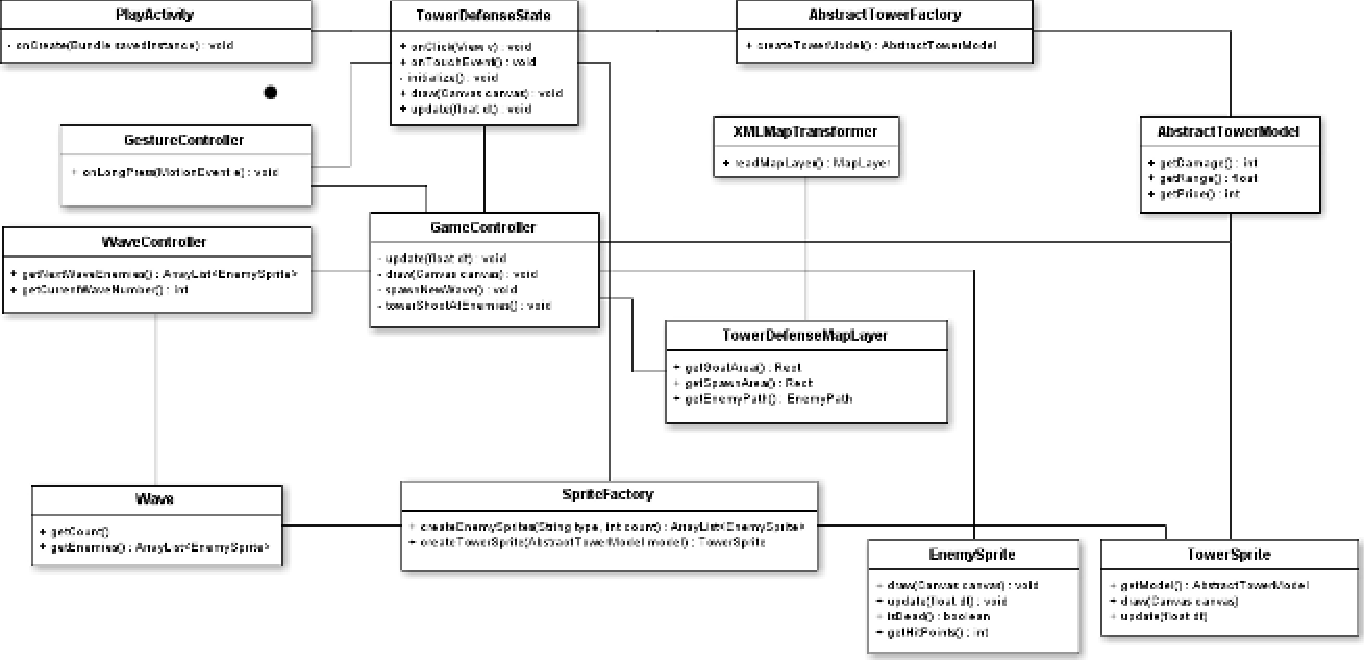
\includegraphics[width=1\linewidth]{main/figures/logicalview}
		\caption{Class diagram over the most important components}
		\label{fig:structure}
\end{figure}



\bibliographystyle{plain}
\bibliography{ref}
\end{document}
